\documentclass[conference]{IEEEtran}
\IEEEoverridecommandlockouts
% The preceding line is only needed to identify funding in the first footnote. If that is unneeded, please comment it out.
\usepackage{cite}
\usepackage{amsmath,amssymb,amsfonts}
\usepackage{algorithmic}
\usepackage{graphicx}
\usepackage{textcomp}
\def\BibTeX{{\rm B\kern-.05em{\sc i\kern-.025em b}\kern-.08em
    T\kern-.1667em\lower.7ex\hbox{E}\kern-.125emX}}
\begin{document}

\title{The evolutionary race: improving the process of evaluating car
 controllers in racing simulators}
%\title{Evolved to win: improving the process of evaluating car
%  controllers in racing simulators}
%\title{The evolutionary race: generating enhanced fuzzy controllers for TORCS}
% Antonio - Check this new title, I have had an inspiration moment. ;D


%\thanks{This work has been supported in part by: Ministerio espa\~{n}ol de
%Econom\'{\i}a y Competitividad under project TIN2014-56494-C4-3-P
%(UGR-EPHEMECH), TIN2017-85727-C4-2-P (UGR-DeepBio) and TEC2015-68752 (also funded by FEDER).}
%}

\author{\IEEEauthorblockN{Mohammed Salem\IEEEauthorrefmark{1},
Antonio M. Mora\IEEEauthorrefmark{2},
Juan J. Merelo\IEEEauthorrefmark{3} and
Pablo Garc{\'i}a-S{\'a}nchez\IEEEauthorrefmark{4}}
\IEEEauthorblockA{\IEEEauthorrefmark{1}Department of Computer Sciences, University of Mascara, Algeria. \\Email: salem@univ-mascara.dz}
\IEEEauthorblockA{\IEEEauthorrefmark{2}Department of Computer Sciences and Technology, ESIT, International University of La Rioja (UNIR), Spain. \\Email: antoniomiguel.mora@unir.net}
\IEEEauthorblockA{\IEEEauthorrefmark{3}Dept. of Computer Architecture and Computer Technology. University of Granada, Spain. \\Email: jjmerelo@geneura.ugr.es}
\IEEEauthorblockA{\IEEEauthorrefmark{4}Department of Computer Science, ESI,
University of C{\'a}diz, Spain. \\Email: pablo.garciasanchez@uca.es}
}

\maketitle

\begin{abstract}
Simulated car races have been used for a long time as an environment
where car controlling algorithms can be tested; they are an
interesting testbed for all kind of algorithms, including
metaheuristics such as evolutionary algorithms; however, the challenge
in these evolutionary algorithms is to design a reliable and effective
evaluation process for the individuals that eventually translates into
good solutions to the car racing problem: finding a controller that is
able to win in a wide range of tracks and with a good quantity of
opponents. Evaluating individual car controllers involves not only the design of a proper fitness function representing how good the car controller would be in
a competitive race, but also the selection of the best solution for the
optimization problem being solved; this decision might not be
easy when uncertainty is present in the problem
environment; in this case, weather and track conditions as well as unpredictable
behavior of other drivers. 
Creating a methodology for the automatic design of  the controller of an
autonomous driver for a car racing simulator such as TORCS is an
optimization problem which offers all these challenges. Thus, in this
paper we describe an analysis and some proposals to improve the
evaluation of optimized fuzzy drivers for TORCS over previous attempts
to do so. It builds on preliminary results obtained in previous papers as a baseline and aims to obtain a more competitive autonomous driver via redesign of the fitness evaluation procedure; to this end, two different fitness functions are studied in several experiments, along with a novel competition-based approach for the selection of the best individual in the evolution. 
% Antonio - Complete this with the obtained results and conclusions
% I don't know if different approaches are eventually used. Erase if not.
% Antonio - just one approach: the score-based
\end{abstract}
\begin{IEEEkeywords}
Videogames, fuzzy controllers, TORCS, Steering control, Optimization,
Genetic Algorithms, car racing games
\end{IEEEkeywords}
%%%%%%%%%%%%%%%%%%%%%%%%%%%%%%%   INTRODUCTION   %%%%%%%%%%%%%%%%%%%%%%%%%%%%%%%
%
\section{Introduction}
\label{sec:intro}

Autonomous driving is a problem that shows up in many environments,
including of course self-driving cars, but also in drones, ships,
trains and underwater vehicles. In general, there will be a series of
sensor inputs that include real speed, obstacles and other vehicles,
and based on those sensors, the bot will have to take a decision on
speed and steering that is optimal in several different
senses \cite{Autodriv2006}. Testing different autonomous driving methodologies in real life is usually reserved to just a few big players, and methodologies
as well as algorithms are usually tested in simulated environments;
these simulated environments, at the same time, offer the incentive of
competition among your system and others. In this paper, we will be
using the Open Racing Car Simulator (TORCS) \cite{WebTORCS} is a very
realistic racing simulator which offers a great testbed for the
implementation and evaluation of autonomous drivers.  
It has been used several times for the celebration of Artificial
Intelligence (AI) competitions, where the aim is to create the best
autonomous driver for racings
\cite{torcs5,manualTORCS,Torcs3,torcs7,oponnents2010}. Besides being
able to test your car against other cars that have been published, it
can be used as a standalone environment to optimize driving in a
solo race. 

Evolutionary Algorithms (EAs) \cite{EAs_Back96} have been frequently
applied as a general-purpose optimization method in this area,
generally combined with behavioural engines that rule different parts
of the car
\cite{Floreano2004,CarRacing_Pelta09,SAES2012,QuadfliegMO,torcs2012}. These
driving engines have included lately fuzzy controllers
\cite{Guadarrama2008, LFAG, PerezEvolvingFuzzy09}. These controllers
use fuzzy Logic \cite{Fuzzy2011}, a  technique that is quite suitable
for defining this kind of autonomous agents, since they are in part
inspired by the human reasoning when driving. A fuzzy controller works
with linguistic variables, and will for instance turn {\em slightly}
to the right when the next curve is {\em close}, but these controllers
have to be designed to map properly input to desired outputs in
particular situations. Previously, the authors presented an approach
combining two specialized fuzzy controllers, designed by hand, that
were able to decide the car's proper steering angle and desired speed
at every single point (or tick) during a race \cite{evo17}. This
driver was later improved \cite{evo18} optimizing the parameters of
their membership functions by means of a Genetic Algorithm
\cite{GAs_Goldberg89}; this automated design improved manual one
obtaining several controllers that were able to beat the initial
hand-designed controller in a race, as well as other published
controllers. 

This proved that evolutionary algorithms were able to get the fuzzy
controller parameters better than a hand-made design, but at the same
time revealed several challenges. In general, evolutionary algorithms
optimize the fitness function that is used; evolved fuzzy controllers
(hereafter FCs) will be eventually as good as the fitness function allows. 
But in this particular case we cannot use as fitness function the position
obtained by the FC in every possible race on every possible track with
every possible opponent, so we have to settle for a {\em surrogate} of
the fitness in a very limited environment. First we opted for
eliminating opponents and making evaluations in solo races; then we
chose a particular track that combined straight segments as well as
some curves and did not take too long to run, and eventually we had to
decide what factors related to speed, damage and lap time were going
to be effectively included in the final fitness function. 

Results were encouraging, but it is still a surrogate model. As such a
model, we need to decide on the best track to perform {\em training}
and also the solo race measures with the biggest impact in the
eventual racing performance. This is why in this paper we have
combined into the fitness function only those terms related with speed during race (to maximize) and damage (to minimize) - the most important factors - in two different approaches.
Besides, the fitness evaluation process has a certain amount of uncertainty because damages and some track conditions can randomly vary in different
evaluations. This is why instead of selecting directly the driver as
we did before, we will be using an actual race among the best drivers
to select the best one.

The main objective of the three new techniques introduced in this
paper, namely, heuristic track selection, fitness function design and
{\em winner} selection have as the main objective to create a better
model of the racing environment. Its results will be commented in the
corresponding section. 

%considering the noisy nature of the problem, which leads to the fact
%that the same individual could obtain very good or very bad results in
%the same races, and against the same opponents, due to the
%stochasticity present in the game and in the rivals' AI.
% Antonio - Just in case we want to comment something about te uncertainty/noise of the game


% Antonio - comment on the results

%Once optimized, the best genetic-fuzzy based controllers (one per fitness) have been evaluated in a practice race (without rivals) first, and then in a real race against different drivers in TORCS. 
%According to the obtained results the enhanced controllers perform both much better than the original fuzzy controller, improving the lap time and reducing the received damage. Moreover they are much more competitive against tough rivals, reaching high ranks in the most difficult races.

% Antonio - describe the final paper structure
The rest of the paper is organized as follows. Next we present the
state of the art, to be followed by a description of the TORCS
simulator, the fuzzy controllers and the Genetic Algorithm implemented in Section \ref{sec:experimental_setup}. After it, the experiments conducted and the obtained results are described in Section \ref{sec:results}. Finally, conclusions and future lines of work will be presented in section \ref{sec:conclusions}.


%%%%%%%%%%%%%%%%%%%%%%%%%%%%%%  STATE OF THE ART  %%%%%%%%%%%%%%%%%%%%%%%%%%%%%%
\section{State of the Art}
\label{sec:soa}

TORCS has become one of the main environments for research on AI since its launch in 2007 \cite{WebTORCS}. It offers different kind of problems to solve, such as the definition of the optimal parameters for the cars (before the race) \cite{Kole-ParamCarTunning12}, and the main one, which is the design of competitive autonomous drivers aiming to win races against other cars, mainly presented in the context on the Simulated Car Racing Competition \cite{SimulatedCarRacing-2008}.

Evolutionary algorithms have targeted TORCS almost since its
publication, for instance, for determining the
optimal trajectory of a lap in a known circuit \cite{drivingGA2008},
but this approach suffers from the problem that the obtained
trajectory in the evolving process strongly depends on the initial
state of the car.  
In the same context, the authors in \cite{GaRaceLine2010} tried to design a novel approach to compute the optimal racing line without any human intervention, using a GA to find the best trade-off between
the minimization of two conflicting objectives: the length and
the curvature of the racing line.

However, definitely, the most prolific area of application of EAs
inside TORCS has been the optimization of autonomous controllers for
car driving, i.e. conducting a meta-optimization process. 
Thus, EAs have been applied to `refine' the parameters which define
the driver's behavior \cite{ButzCMAES09,SAES2012}, or to improve the
structure/architecture of the models \cite{evol,neurone}, working
offline, or online (during the game)
\cite{TanOnline08,Cardamone_Online_NN}.
% FUZZY + EAs
Our approach is focused in this line, proposing the application of an off-line genetic algorithm for the improvement of the parameters which determine the behavior of a controller for TORCS. We have focused on a Fuzzy-based model, as it is one of the best options for modeling human-like decisions and actions, as others authors have also used this kind of technique in the literature with good results \cite{torcs2012}. 
For instance, in \cite{Guadarrama2008}, a fuzzy rule-based car controller for a Car Racing Competition was built and tuned with co-evolutionary genetic algorithms. Two fuzzy sub-controllers were designed (acceleration and turning angle). But this approach was applied to a simpler simulator than TORCS which is a more realistic and time-constrained simulator. 

P{\'e}rez et al. introduced an evolutionary fuzzy approach for TORCS in \cite{PerezEvolvingFuzzy09}, where they applied EAs for improving fuzzy models to infer the acceleration and turning angle. However, the models were not so specialized as the proposed here, since their controller did not compute the target speed, which is a key factor for a competitive controller. 

Onieva et al. \cite{LFAG} presented a parametrized modular architecture with a fuzzy system and a GA, aiming to reproduce the behavior of a human driver when controlling the steering wheel. In this line, we presented an improved approach \cite{evo17}, which evolved a fuzzy-based driver considering the target speed in addition to the steer (two fuzzy sub-controllers).
This controller was also enhanced in a further work \cite{evo18} optimizing the parameters of the membership functions by means of a real coded genetic algorithm, obtaining a noticeable improvement in performance.

In this paper we focus on the improvement of the evolved controllers by means of a redefinition of the fitness functions, looking for a parameter-less approach (no weights in the terms) \cite{Harik-ParameterLess99}, which will be also more focused on the real objectives of a driver during a race, rather than the overall objective. In addition, a `fairer' selection process of the best individual has been implemented, aiming to focus on real good drivers in races, instead of choosing the one with the highest fitness value, which could have a poorer performance due to the noise of the problem.



%%%%%%%%%%%%%%%%%%%%%%%%%%%%%%  TORCS  %%%%%%%%%%%%%%%%%%%%%%%%%%%%%%

\section{Experimental Setup}
\label{sec:experimental_setup}

The Open Racing Car Simulator (TORCS) \cite{WebTORCS} is an open
source, modern, multi-player, modular and portable racing simulator
that allows users to compete against other computer-controlled opponents.
Its high degree of modularity and portability, together with the
realistic and real-time driving simulation, make it an ideal testbed
for artificial intelligence research, as we have shown in the previous section.

Every car in TORCS includes  a large set of sensors \cite{Torcs3},
whose values the car can use during a race, such as distances to track borders, to rivals, current fuel, current gear, position in the race, speed, or damage, among others.
The sensor values are considered by any TORCS autonomous driver, or
{\em controller}, to manage the car using actuators \cite{Torcs3}: the
steering wheel, the accelerator, the brake pedal and the gearbox.   

%Thus, a controller is a program, running inside TORCS, that drives a car automatically. It gets as input information about the current state of
%the car and its situation on the track (sensors). These collected data
%are used to decide actions to perform in the next simulation tick.  


\subsection{Fuzzy sub-controllers}
\label{subsec:subcontrollers}

%*****************************  FUZZY CONTROLLER  ******************************
The controller proposed initially \cite{evo17} has the same modular
architecture as the simple TORCS driver; however, the target speed and
steering angle are computed by means of two modular and specialized
fuzzy sub-controllers, which consider five position sensors. This is
the controller which will be improved by means of a GA in this
work.

The {\em fuzzy target speed sub-controller} aims to estimate the
optimal target speed of the car, both in straight parts and curves of
the track, taking into account two criteria: move as fast as possible
and be safe. This estimation is based on two general cases: if the car
is in a straight line, the target speed will take a maximum value
(\textit{maxSpeed} km/h). However, if it is close to a curve, the
controller will decrease the current speed to a value included in the
interval \textit{[minSpeed, maxSpeed]} km/h. 

This fuzzy controller has an output, the speed, and three input values:
\begin{itemize}
	\item Front = Track\_9: front distance to the track border (angle 0º).  
	\item M5 = max (Track\_8, Track\_10): max distance to the track border in an angle of +5º and -5º with respect to Front.
	\item M10 = max (Track\_7, Track\_11): max distance to track border in an angle of +10º and -10º.
\end{itemize}

It is a Mamdani-based fuzzy system \cite{iancu2012} with three
trapezoidal Membership Functions (MF) for every input variable. 
%The description of these fuzzy inputs and output are represented in Table
%\ref{tab:flouevar}. 
In \cite{evo18} the different sets of parameters which define the membership functions were improved using a Genetic Algorithm to obtain the best results.

%\begin{table*}
%	\centering
%	{\scriptsize
%		\caption{Fuzzy variables description.}
%		\label{tab:flouevar}
%		\begin{tabular}{ |p{1.5cm}|p{2cm}|p{2cm}|p{2 cm}|p{1 cm}|p{1.5 cm}|p{1.5 cm}|}
%			\hline
%			{ \textbf{Variable}}&
%			{ \textbf{Range}}&
%			{ \textbf{Name}}&  
%			{ \textbf{MF}} &
%			{ \textbf{Low}} &
%			{ \textbf{Medium}}&
%			{ \textbf{High}} \\
%			\hline
%			Input & [0-100] m & Front & trapezoidal & [0-50] & [20-80] & [60-100]
%			\\
%			\hline
%			Input & [0-100] m & M5 & trapezoidal &[0-40] & [10-70] & [50-100] 
%			\\
%			\hline
%			Input & [0-100] m  & M10 & trapezoidal & [0-30] & [20-60] & [50-100]
%			\\
%			\hline 
%			Output & [0-200] m/s & TargetSpeed & singleton & / & / & /
%			\\
%			\hline 
%		\end{tabular} 
%	}
%\end{table*}

% This is from the last paper? If so, just a reference would be
% enough. We need to save space - JJ
% Consider whether adding this again or not -- JJ
% Antonio - not needed

Moreover, the controller is based in a set of fuzzy rules, designed to maximize the car speed depending on the distance to the track border. These rules can be consulted in \cite{evo17}.
% Antonio - TODO: Include the rules if there is available space?

%The fuzzy rules are:

% \begin{itemize}
% {\small
% 	\item \texttt{IF Front is High THEN TargetSpeed is TS1}
% 	\item \texttt{IF Front is Medium THEN TargetSpeed is TS2}
% 	\item \texttt{IF Front is Low and M5 is High THEN TargetSpeed is TS3}
% 	\item \texttt{IF Front is Low and M5 is Medium THEN TargetSpeed is TS4}
% 	\item \texttt{IF Front is Low and M5 is Low and M10 is High THEN TargetSpeed is TS5}
% 	\item \texttt{IF Front is Low and M5 is Low and M10 is Medium THEN TargetSpeed is TS6}
% 	\item \texttt{IF Front is Low and M5 is Low and M10 is Low THEN TargetSpeed is TS7}\\
% }

% In addition, a crisp rule is added to obtain a maximum value of the target speed when the three input variables are as big as possible:\\
% {\small	
% \item \texttt{IF Front = MAXDISTSPEED or M5 = MAXDISTSPEED or M10 = MAXDISTSPEED THEN TargetSpeed = MAXSPEED}
% }
% \end{itemize}

% MAXDISTSPEED is the longest possible value for the track sensors, and MAXSPEED is the maximal speed for the specific car. 
% The output value is encoded by seven singletons TS1 to TS7, being respectively: 280, 240, 220, 180, 120, 60 and 30.\\


% %***********************************************
% \noindent
% \textbf{Fuzzy steering control sub-controller}\\
% %

The second is the {\em fuzzy steering sub-controller}, which aims to define the steer angle estimating and determining the target position of the car. 

The structure of this sub-controller is similar to the speed one, but it has the steering as output. Thus, the set of sensors considered is the same as in the speed case.

Then, as general rules: if the car is in a straight line, it will set as target position half width of the race track (central position of the lane). Whereas, if the car is near a right curve, it will approach the path leading to the right, with a space between the car and the border of the track to avoid the loss of control. The same approach is considered if the car is near a left curve.

In order to detect the curves, the controller focuses on the sensor values (M10, M5, and Front). So, if the value on Front sensor is the longest, there is a straight road; whereas if the values of M5 and M10 with positive angles (+5 and +10) are the longest, there is right curve; and the other way round.

It uses a base of rules which has been defined trying to model the behavior of a human driver \cite{evo17}.

%, so, for this controller:
% Antonio - TODO: Include the rules if there is available space?

% {\small
% \begin{itemize}		
% 	\item \texttt{IF Front is High THEN steer is S1}
% 	\item \texttt{IF Front is Medium AND M10 is High THEN  steer is S2}
% 	\item \texttt{IF Front is Medium AND M10 is Medium AND M5 is Medium THEN steer is S2}
% 	\item \texttt{IF Front is Medium AND M10 is Medium AND M5 is Low THEN steer is S3}
% 	\item \texttt{IF Front is Low AND M10 is High THEN steer is S3}
% 	\item \texttt{IF Front is Low AND M10 is Medium AND M5 is Medium THEN steer is S4}
% 	\item \texttt{IF Front is Low AND M10 is Medium AND M5 is Low THEN steer is S4}
% \end{itemize}	
% }

% The values for S1 to S4 are respectively: 0, 0.25, 0.5, and 1.
% When M10=Track[7] we will take negative values of the steer (steer=-steer).

% These controllers were defined with our own criteria, but they could be far from being optimal, so, in the following section we apply a Genetic Algorithm for their improvement.


%%%%%%%%%%%%%%%%%%%%%%%%%%%%  OPTIMISING WITH GAS  %%%%%%%%%%%%%%%%%%%%%%%%%%%%

\subsection{Genetic Algorithm}
\label{subsec:GA_optimization}

% Designing an optimal fuzzy controller for TORCS racing needs a human expert to define the membership functions parameters and the rule base. This expert, even if he exists, could not provide an exact repartition of the fuzzy membership functions values over the universe of discourse. 

% This difficulty have led us to move towards the use of Genetic Algorithms  \cite{GAs_Goldberg89} because of their global exploration characteristic in a complex environment, as this problem plots. 

The proposed optimization approach aims to find the optimal parameters of the membership functions of the two sub-controllers previously introduced. 
The followed process is depicted in Figure \ref{fig:ga}, in which, as it can be seen, the GA uses TORCS for the evaluation of every individual during the evolutionary process.
\begin{figure}[!ht]
  \label{fig:ga}
  \begin{center}
    \includegraphics[width=10cm]{fig/flowchart}
  \end{center}
  \caption{Optimization of a fuzzy controller flowchart. The evaluation of an individual is performed by: putting the parameter values on the two sub-controllers, launching a race in TORCS with this configuration, obtaining the resulting values of Damage, Top Speed and mean Lap Time and using these values for the computation of the fitness of the individual.}
\end{figure}	
The GA starts by creating the initial population with random values
for the parameters in the defined range $[0,100]$. The fitness of each
candidate solution is computed by injecting its gene values to the
parameters of the membership functions of the two fuzzy
sub-controllers. The defined autonomous controller is used to drive a
car in a 20 laps race in a circuit without opponents, and the
results (Top speed, Damage and Mean Lap time) are used to compute the
fitness value. 

%***********************************************

As previously stated, the designed fuzzy controllers have trapezoidal membership functions given by Equation \ref{eq:trapmf}.
In such a controller, fuzzy rules are applied to linguistic
terms. These terms, which qualify a linguistic variable, are defined
through membership functions, which, in turn, depend on a set of
parameters that `describes' their shape (and operation). Using a GA we
will optimize the parameters of the membership functions that
constitute the fuzzy partition of the linguistic variable
\cite{ThangG08}. The input linguistic variables in our problem,
\textit{Front, Max5} and \textit{Max10}, are represented by three
trapezoidal membership functions. 

%(See Table \ref{tab:flouevar}). % Maybe reduce? I think these two sentences could be merged into one


A trapezoidal membership function in a finite universe of discourse \textit{[a, b]} can be defined by:

\begin{equation}
\mu_{A}(x)= \left \{
\begin{array}{ll}
\frac{x - x_{1}}{x_{2} - x_{1}},& x_{1} \leq x \leq x_{2}\\
1 , &x_{2} \leq x \leq x_{3}\\
\frac{x_{4} - x}{x_{4} - x_{3}},& x_{3} \leq x \leq x_{4}\\
0        ,& else\\	
\end{array}
\right.
\label{eq:trapmf}
\end{equation}
with:
\begin{equation}
x_{1} \leq x_{2} \leq x_{3} \leq x_{4}
\end{equation}
This MF function is defined by four parameters $x_{1}$, $x_{2}$,
$x_{3}$ and $x_{4}$ taking their values in the interval \textit{[a,
  b]}.% (See Figure \ref{fig:trapeze}).

\begin{figure}[!ht] 
	\begin{center}
		\includegraphics[scale=0.7]{fig/trapese}
		\caption {Trapezoidal MFs}
		\label{fig:trapeze}
	\end{center}
\end{figure}
And a fuzzy partition with \textit{n} trapezoidal membership functions
is defined by \textit{2n} variables (\textit{a =} $ x_{1}$,$x_{2}
$,. .., $x_{2n} $ \textit {= b})(Equation \ref{eq:e1}). In this case,
the representation is given by the
figure \ref{fig:at} 
\begin{figure}[!ht] 
	\begin{center}
		\includegraphics[scale=0.55]{fig/trapezoidal.png}
		\caption {Trapezoidal-shaped MFs coding}
		\label{fig:at}
	\end{center}
\end{figure}
with:
\begin{equation}
a = x_{1} \leq x_{2} \leq...\leq x_{2n-1} \leq x_{2n}=b 	
\end{equation}		

\begin{equation} 
\begin{tabular}{l}
$\mu_{A1}(x)=  \left \{
\begin{array}{ll}
1, &x_{1} \leq x \leq x_{2}\\
\frac{x_{3} - x}{x_{3} - x_{2}}, &x_{2} \leq x \leq x_{3}\\
0        , &x > x_{3}\\
\end{array} 
\right.$		\\ 	
$\mu_{Ai}(x)= \left \{
\begin{array}{ll} 
0, &x \leq x_{2i-2}\\
\frac{x - x_{2i-2}}{x_{2i-1} - x_{2i-2}}, &x_{2i-2} \leq x \leq x_{2i-1},n=2,...,i-1\\
1, & x_{2i-1} \leq x \leq x_{2i}\\
\frac{x_{2i+1} - x}{x_{2i+1} - x_{2i}},& x_{2i} \leq x \leq x_{2i+1}\\
0  , &x > x_{2i+1}\\
\end{array}  
\right.	$		\\
$\mu_{An}(x)= \left \{
\begin{array}{ll} 
0, &x \leq x_{2n-2}\\
\frac{x - x_{2n-2}}{x_{2n-1} - x_{2n-2}},& x_{2n-2} \leq x \leq x_{2n-1}\\
1 ,& x > x_{2n-1} 
\end{array} 
\right.$\\
\label{eq:e1}
\end{tabular}
\end{equation}

% As we have just seen, a linguistic variable is represented by a number
% of parameters that depend both on the number and type of used
% membership functions  \cite{ThangG08}. Also the choice of coding to
% use for these different parameters depends both on the desired
% precision on the values and on their range of values. 
% I don't think this paragraph is needed - JJ
%  Mohammed:  tell me that you left the results section , You haven't removed it  too JJ jeje

When the number of parameters is reduced and their ranges of variations are well defined, a GA with a binary coding is largely sufficient to find their optimal values. On the other hand, if the number of parameters becomes important, and their variation interval is not well known, the real coding is the most appropriate \cite{elsayed13}. 
Since our work requires some precision and the variation interval of
each parameter is not well known, we have considered a real coding
implementation in a vector that includes all variables to optimize.

In that GA, every individual is a vector of 18 values/parameters, 6 per variable. Figure \ref {fig:cromosome} illustrates the structure of the chromosome.
\begin{figure*}[!ht]	
  \begin{center}
    \includegraphics[width=12cm]{fig/chromosome2.png}
    \caption{Chromosome description}
    \label{fig:cromosome}	
  \end{center}	
\end{figure*}

The initialization of the chromosomes (first population) is performed
assigning random values inside a range of variation
\cite{GAs_Goldberg89}, in order to start from feasible values
\cite{evo17}. 
Tournament based selection has been used to elect chromosomes as
parents for genetic operators, while simple arithmetic two point
crossover \cite{crossGA2017} and non uniform mutation
\cite{mutation1997} have been chosen, as two of the most contrasted
methods in the literature. 

%***********************************************


The objective of the car controller is to win as many races as
possible. However, we have to optimize the most general case by
carrying out solo {\em training races}, which will be less sensitive to the presence of noise/uncertainty due to the participation of other controllers.

In previous approaches we focused on minimizing the damage of
the car ($damage$) and the lap time $LapTime$, while
maximizing $TopSpeed$. However in this study, we have turned our focus and have considered:
\begin{itemize}
\item $MinSpeed$: aiming to increase the good driving in the difficult zones of the tracks (e.g. curves).
\item $MaxSpeed$: centered on the enhancement of the controller in easy or straight parts.
\item $AVG(Speed)$: which shows the combination of the overall behaviour in the whole track.
\item $Damage$: aiming to create `safe' controllers, as it is mandatory being able to finish the race.
\end{itemize} 
%
We have combined these terms into two possible fitness functions:

\begin{description}
	\item[GFC-MMS:]  
	\begin{equation} \label{fit1}
	\begin{array}{ll}
	f_{1} =   \frac{(MinSpeed*Maxpeed) }{Damage+1}
	\end{array}
	\end{equation}
	\item[GFC-AVS:] 
	\begin{equation} \label{fit2}
	\begin{array}{lll}
	f_{2}= \frac{AVG(Speed)}{Damage+1}
	\end{array}
	\end{equation}	
\end{description} 

As it can be seen, the aim is to maximize the minimum and maximum velocities while minimizing the damage in the first fitness. In the second one, we try to maximize the average speed on the circuit.

To evaluate every candidate controller during the evolutionary process, we will make each of them compete in a 20 laps practice race in a medium difficulty circuit without rivals. As stated, we have omitted the presence of opponents in order to avoid including additional uncertainty sources to the optimization process. In order to obtain general-behaviour controllers, the selected track for this process will be one with a combination of curves and straight parts.

After this practice, the obtained output values $Damage$, $Minspeed$, $MaxSpeed$ and $AVG(Speed)$ are collected to compute the corresponding fitness value.


%%%%%%%%%%%%%%%%%%%%%%%%%%%%  RESULTS  %%%%%%%%%%%%%%%%%%%%%%%%%%%%

\section{Experimental results}  
\label{sec:results}

After analyzing most of the available tracks, we have selected for these experiments the \textbf{Alpine 2} circuit. It is a quite complex one, with multiple turns, but also straight parts (See Figure \ref{fig:alpine2_track}).

\begin{figure}[!ht]	
  \begin{center}
    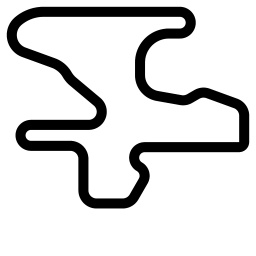
\includegraphics[width=7cm]{fig/alpine2.jpg}
    \caption{Alpine 2 Track: Slow mountain road. Length: 3773.57m, Width: 10m}
    \label{fig:alpine2_track}	
  \end{center}	
\end{figure}

We have used the driving car for our controllers \textit{car1-tbr1}, since according to previous experiments \cite{evo17}, this is a fair choice due to its moderate performance. This will lead our controller to be prepared to drive in the most usual conditions. 

We have evaluated the Genetic Fuzzy Controller (GFC) with the two proposed fitness functions: GFC-MMS (Equation \ref{fit1}) and GFC-AVS (Equation \ref{fit2}), comparing them for racing performance. We have run the  algorithm with population size of 50 individuals. The rest of parameters are: Generations=50, Crossover rate=0.85, Mutation rate=0.1, and 10 different runs per configuration.


%\begin{table}[!ht]	
%		\centering
%{\scriptsize
%		\caption{GA parameters}
%		\label{tab:GA_config}
%		\begin{tabular}{|p{3.6cm}|p{3cm}|}
%			\hline \textbf{Population size} & 50 \\
%			\hline \textbf{Generations} & 50   \\
%			\hline \textbf{Crossover rate$\textit{P}_{\textit{c}}$} &  0.85 \\
%			\hline \textbf{Mutation rate $\textit{P}_{\textit{m}}$} &  0.1   \\ 		
%			\hline          
%		\end{tabular}	
%}
%\end{table}

The two genetic optimization processes have been run in independently. However, as a difference to previous works in which we just selected as the best the individual with the highest fitness value in the last generation, in this study we have aimed to implement a better process, which we expect will yield a more competitive controller.

To this end, for every approach, once the evolutionary process is
finished, the best four individuals have competed together in 5 races
in the \textbf{Alpine 2} track (used in the optimization) and 5 races in \textbf{E-Track 5} track (a new one for them). 
% Antonio - Mohammed, During how many laps are the races performed?
% It would be interesting to add another column with the fitness of
% those chosen - JJ
In order to enhance the selection of the best, another two controllers are picked randomly from the default TORCS bots
% Antonio - Mohammed, are the bots taken from the default ones? Can you select them randomly in the run or have you selected them in advance?
to participate in the race. Moreover, to do it fairer, we have defined a \textit{score}, so the controller which gets the fastest lap or the minimum damage in each race is given 5 points.

The results of these runs are shown in Table \ref{tab:runsresults}.
\begin{table*}[ht]
  \centering
  {\scriptsize % Please explain all columns. What's "best laps"? And
               % "min damage"? - JJ
    \caption{ Obtained Scores on the race-based selection for the two approaches in two different tracks. }
		{
			\begin{tabular}{|c||c|c|c|c|c|c|c||c|c|c|c|c|c|c||c|}
				\hline
				&\multicolumn{7}{c||}{5 races in Alpine 2 track}&\multicolumn{7}{c|}{5 races in E-Track 5}&\\
				\cline{2-16}
Bots	& 		  R1 & 		  R2 & 		 R3 & 		  R4& 		   R5&Best laps&Min damage& R1&R2&R3&R4&R5&Best laps&Min damage&Total\\
				\hline		
$GFC-MMS_1$ &\textbf{25}& 18		 &8			&15			&12        &15 &10&		12&\textbf{25}& 		18&\textbf{25}&		18&10&10&221\\
$GFC-MMS_2$ &12		 &\textbf{25}& 15 		&12			&15			&0&5&8			&15		  &			15&	4	&10&0&0&136\\
$GFC-MMS_3$ &6			 &6			&10			&10			&8			&0&0&15			&10		  &			10&	18	&6&0&5&104\\
$GFC-MMS_4$ &2			 &	8		&4			&4			&      6    &0&0& 10		& 1		  &		 2&1		&2&0&0&40\\
$GFC-AVS_1$ &1			 &4			&6			&2			&	4		&0&0&4		    &2		  &			12&	10	& 4&0&0&49\\					
$GFC-AVS_2$ &15		&10			& 18		&\textbf{25}&18			&5&10&\textbf{25}& 18	  &	\textbf{25} &15&15&5&10&206\\
$GFC-AVS_3$ &10		&2			&1			&6			&	2		&0&0&2			&6		  &			4&	6	&1&0&0&41\\
$GFC-AVS_4$ &4			&1			&2			&1			&	1		&0&0&1			&4	      &		8&	2	&8&0&0&32\\	
$bt1$ 	 &/			&/			&/			&8			&/			&0&0&/			&8		  &			 6&8		&/&0&0&/\\
$inferno1$&18		&/			&12			&/			&/			&0&0&18			&12		  &			/&/		& /& 0&0&/\\			
$berwin2$&8			&15			&/			&18			&/			&0&0&/			&/		&			/&12	&12&5&0&/\\
$berwin3$&/			&12			&/			&/			&\textbf{25}&5&0&4			&/		&			/&/		&\textbf{25}&5&0&/\\
$damned1$&/			&/			&\textbf{25}&/			&10			&0&0&/			&/		& 			8&/		& /&0&0&/\\			
				\hline
				\hline
			
			\end{tabular}
		}\label{tab:runsresults}
	}
\end{table*}

% Antonio - Mohammed, what do the results with "/" mean?
% Couldn't finish, maybe. But you should add the total anyway - JJ

According to the table, the first individual of GFC-MMS and the second of GFC-AVS have won the same number of races but $GFC-AVS_2$ has achieved better results on the races it did not win.
We have to remark that the TORCS bots results are not counted since they only serve to diversify the selection and they do not participate in all the races.
This selection allowed us to choose the best individual on several races and the most stable and thus avoid the selection by tournament where the winner of a single confrontation is chosen.

It could be remarked that the genetic based fuzzy controllers have get all the points of the minimum damage even when they do not win the race, this fact  justify strongly the use of damage in the fitness functions.
The controllers obtained using the first fitness have also collected  the points of the best laps in  five of the ten races. one has to bear in mind that the best lap is the result of a minimum damage and a high MaxSpeed, these two parameters are optimized by the first function. In the same context, the second fitness tries to maximize the speed average  not necessary the MaxSpeed.

The two best genetic based fuzzy controllers obtained in the previous
experiments, one per fitness function, and thus named $GFC-MMS_1$ and
$GFC-AVS_2$, have been tested in a practice races against selected opponents. The two best controllers of our previous paper \cite{evo18}, $EVO1$ and $EVO2$ are also included in the competition.

This evaluation is a like Formula 1 mini championship of 10 races each one for 20 laps where also six bots from TORCS are used to test our controllers. The first 5 races are conducted in \textbf{Alpine 2} track (trained one); and the other 5 races took place in \textbf{E-Track 5} track.

The results are shown in Table \ref{tab:chsresults}:

\begin{table*}[ht]
  \centering
  {\scriptsize
    \caption{ Results of the mini-championship with 10 drivers and ten races in \textbf{Alpine 2} and \textbf{E-Track 5} tracks }
    % Total points should be added, maybe per track. Also highlight,
    % as above, who won. - JJ
    {
			\begin{tabular}{|c||c|c|c|c|c|c|c|c|c|c||}
				\hline
			&\multicolumn{5}{|c|}{\textbf{Alpine 2}} &	\multicolumn{5}{|c|}{\textbf{E-Track 5}}\\
				\hline
				\hline	
				Drivers&{Race 1}&{Race 2}&{Race 3}&{Race 4}&{Race 5}&{Race 6}&{Race 7}&{Race 8}&{Race 9}&{Race 10}\\
				\hline	\hline			
				$GFC-MMS_1$&	25&	10&	18&	12&	10&	18&	12&	15&	15&	12\\
				$GFC-AVS_2$&	15&	18&	25&	15&	15&	25&	18&	18&	12&18\\
				$Tita1$&	4&	2&	1&	2&	2&	4&	2&	1&	4&	6\\
				$Tita2$&	2&	1&	2&	1&	1&	1&	1&	2&	1&	2\\
				$Inferno1$&12&15&	12&	18&	18&	12&	15&	25&	25&	15\\
				$Inferno2$&10&12&	4&	10&	25&	10&	10&	4&	2&	8\\
				$Berwin1$&	18&	25&	15&	8&	6&	8&	8&	6&	10&	10\\
				$Berwin2$	&8&	8&	10&	25&	12&	15&	25&	10&	8&	25\\
				$EVO1$&	6&	6&	8&	4&	8&	2&	6&	12&	8&	4\\
				$EVO2$&	1&	4&	6&	6&	4&	6&	4&	8&	6&	2\\
				\hline
				\hline
				
			\end{tabular}
		}\label{tab:chsresults}
	}
\end{table*}



From the table, we can see that the fuzzy controllers optimized by the
GA yield best results, obtaining very good overall rankings in the races, We can also see that our two  genetic based fuzzy controllers have win  only one race for 	$GFC-MMS_1$ and two for $GFC-AVS_2$ controller compared to $berwin2 $ and $inferno1$ bots which win three races each one.

This lack of race winning did not stop our genetic controllers from finishing in the first four rankings in the races, which helped them to win the points championship.
This result is due to the trade-off between the damage and the average speed achieved by the fitness function. This property has given our controller an advantage in minimizing damage and looking for top speed in the straight sections of the track while it tries to find the best trajectory in turns to avoid hitting the track edges or get out of it.
The overall number of points of the championship is presented in Figure \ref{fig:points} while Figure \ref{fig:damspeed} represent the numbers of races where each controller has obtained the minimum of damage and the higher MaxSpeed.



\begin{figure*}[h!tb]	
  \begin{center}
    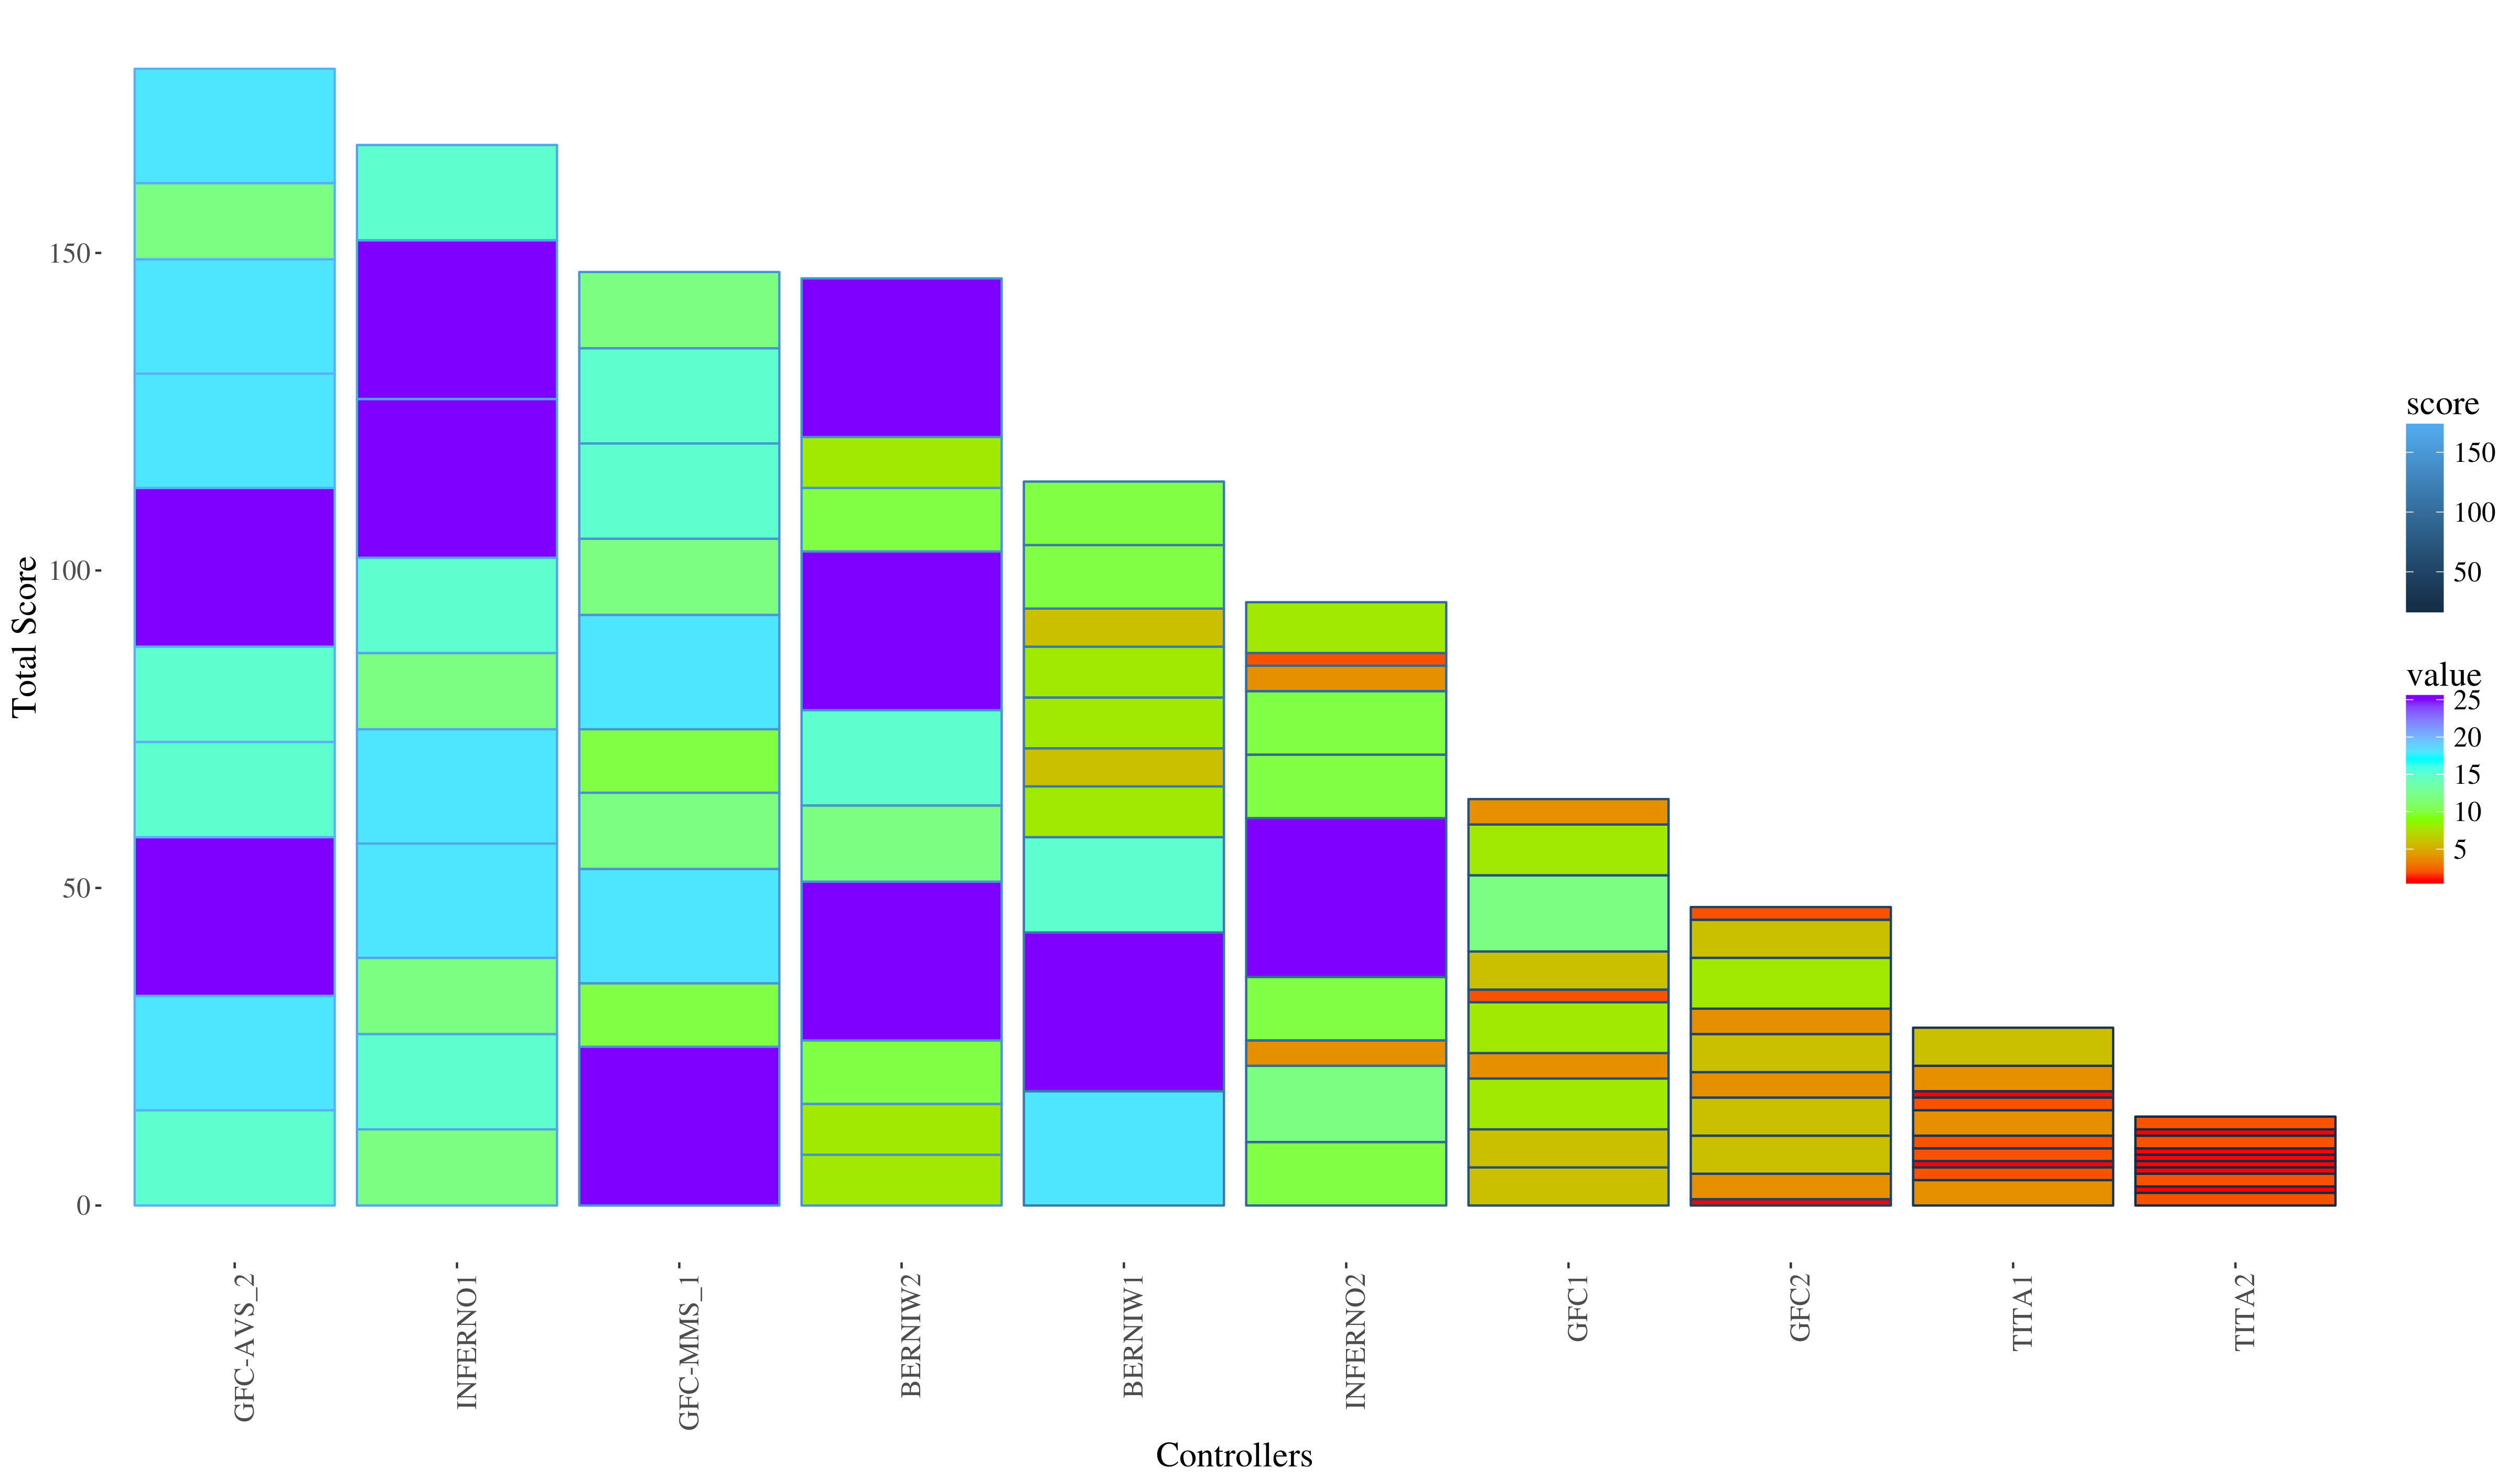
\includegraphics[width=0.95\textwidth]{fig/POINTS.png}
    % Generated with plot-points.R 
    \caption{Total and partial score for all controllers in the {\em
        championship}. {\tt GFC} are the two controllers introduced in
    this paper.}
    \label{fig:points}	
  \end{center}	
\end{figure*}
%
\begin{figure}[!ht]	
	\begin{center}
          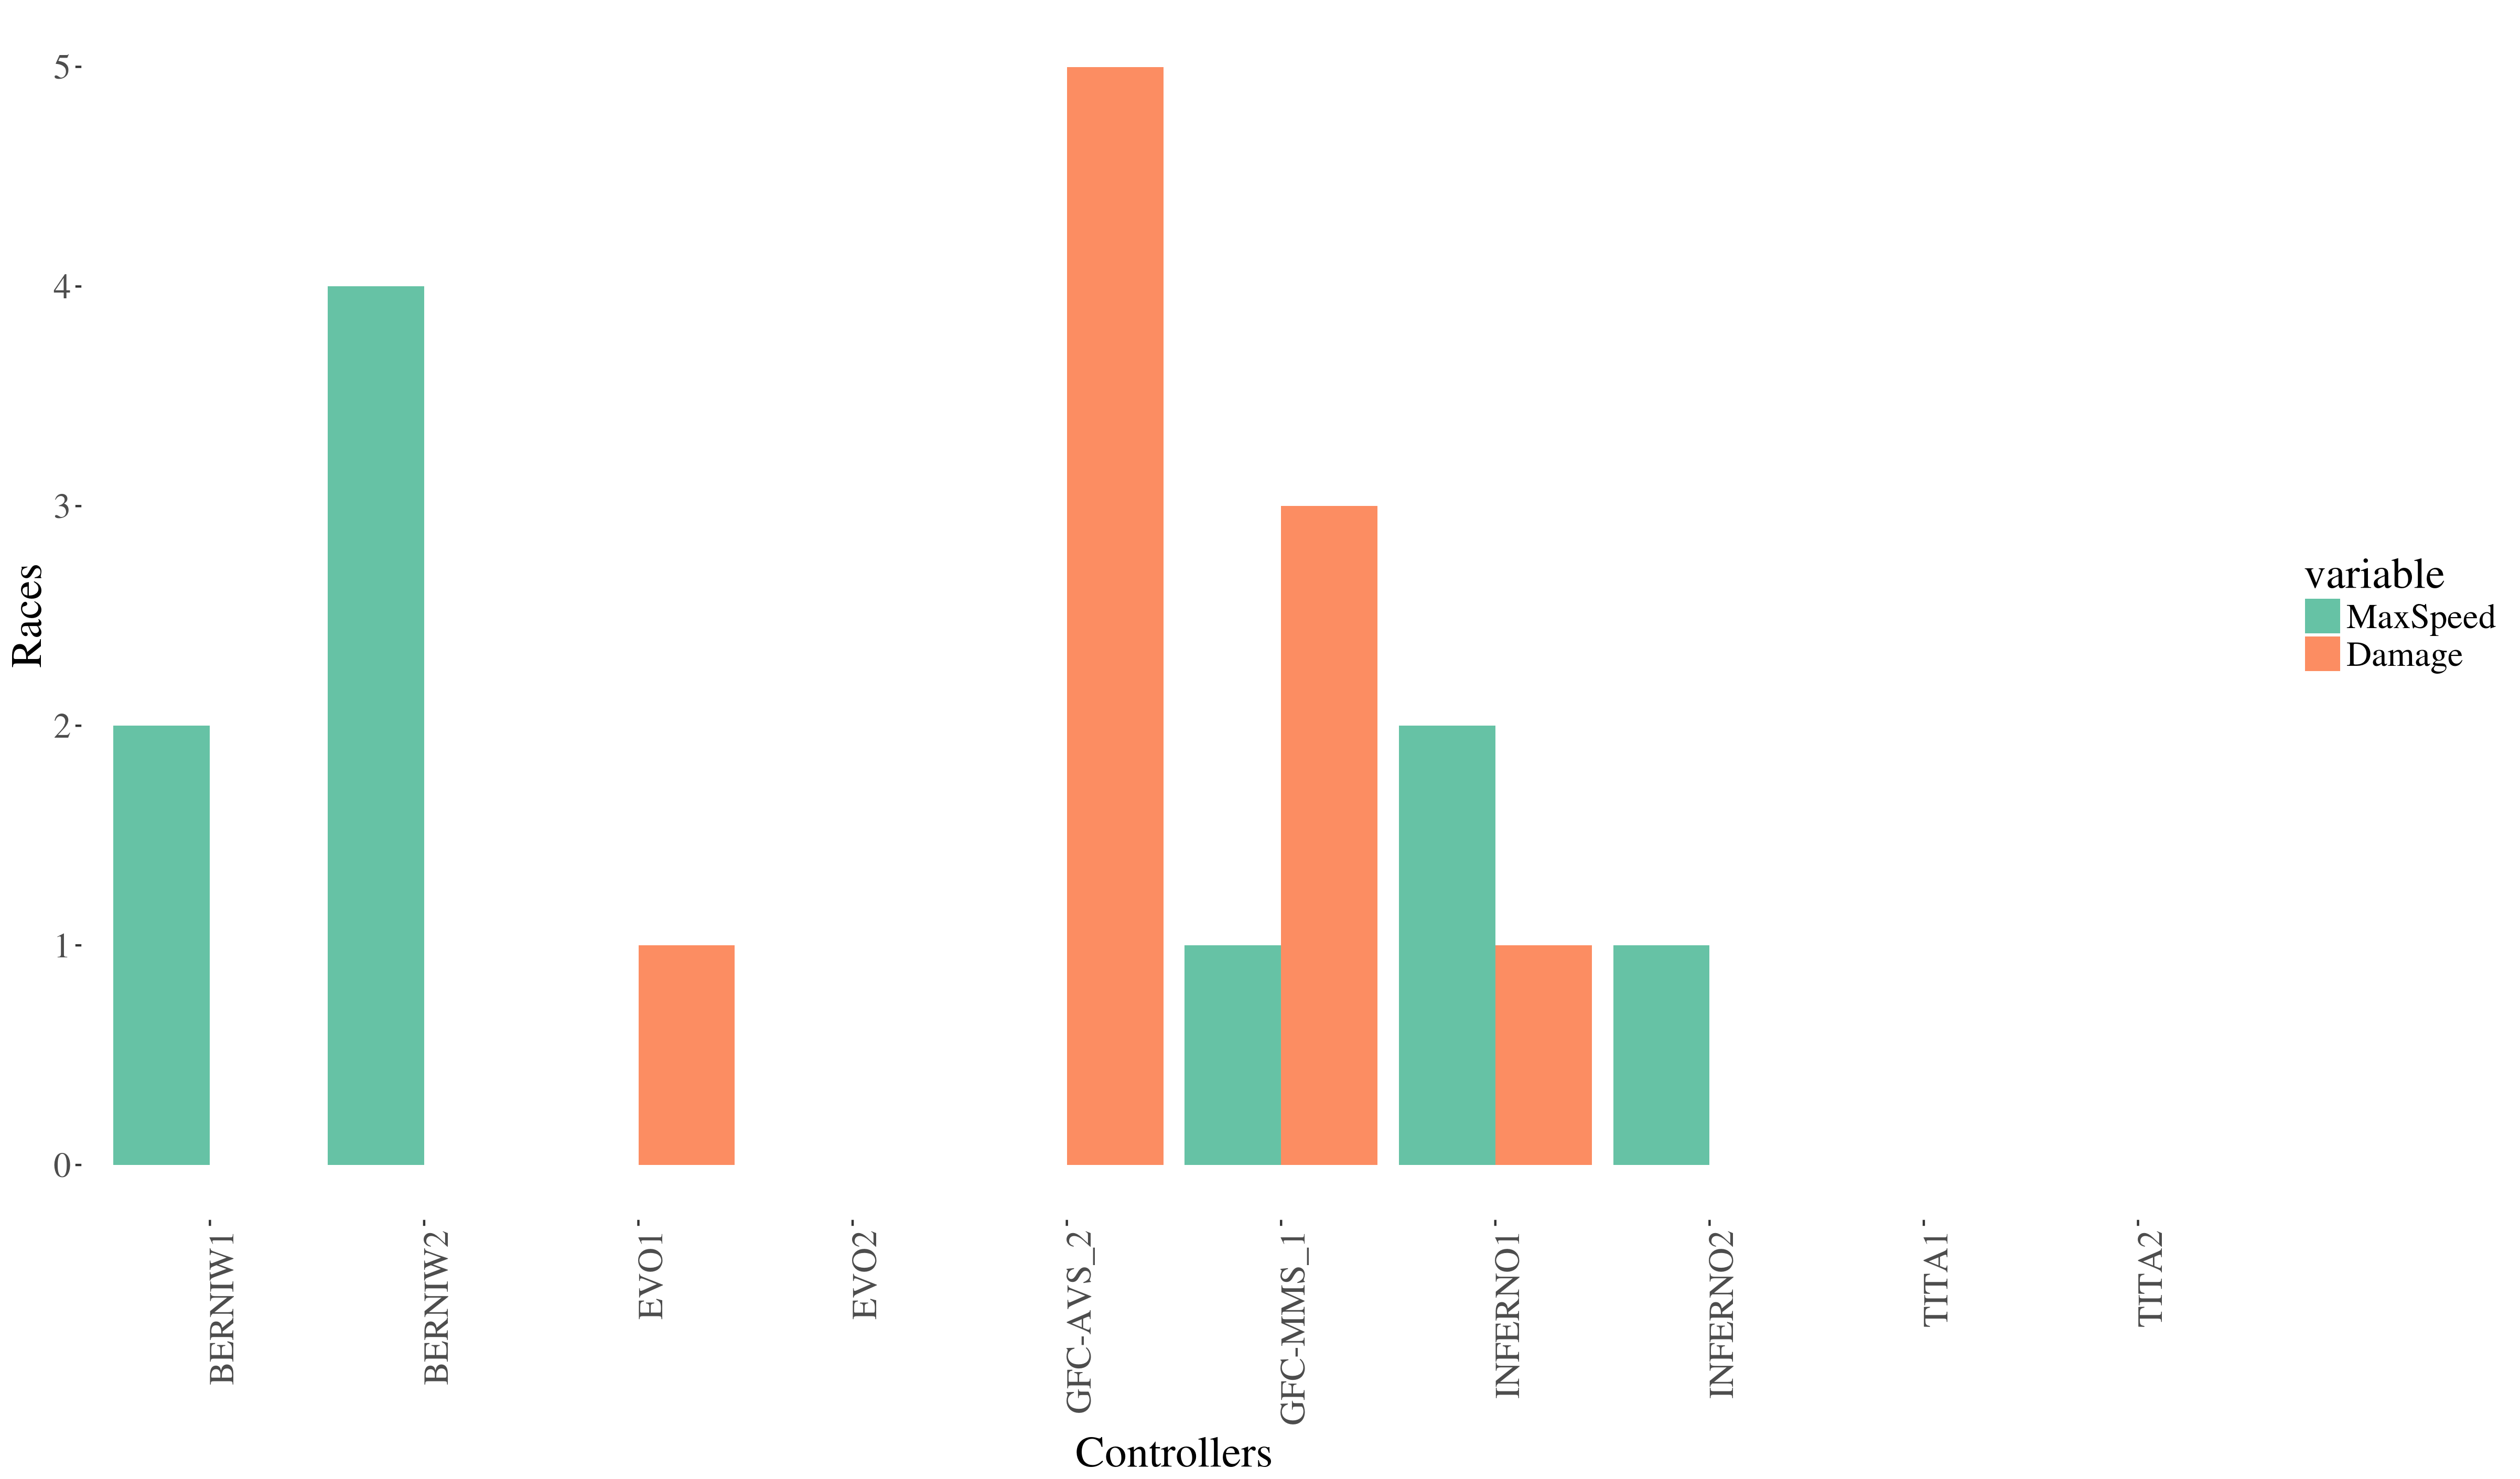
\includegraphics[width=8cm]{fig/HISTSD.png}
          % Plotted with plot-speed-damage.R
		\caption{Chart with number of races where controlled
                  cars are  damaged and where they obtain the MaxSpeed
                in a lap.}
		\label{fig:damspeed}	
	\end{center}	
\end{figure}

Table \ref{tab:damagespeed} presents a comparison between the genetic based fuzzy controllers presented in this paper, \textbf{$GFC-MMS_1$} and \textbf{$GFC-AVS_2$} with  
those of  \cite{evo18}: $EVO1$  and $EVO2$. The average values of $damage$, $MaxSpeed$ and $Speed$ of the ten races in the \textbf{Alpine 2} and  \textbf{E-Track 5} tracks.



\begin{table}[!ht]
  \centering
  {\scriptsize
    \caption{Average damage and Speed Results of GFC in a 5 races in \textbf{Alpine 2} and  \textbf{E-Track 5} tracks}
    \label{tab:damagespeed}
    \begin{tabular}{|p{1.65cm}|c|c|c|c|}
      \hline 
      \multicolumn{5}{|c|}{\textbf{Alpine 2}}  \\	
      \hline  
   & \textbf{$GFC-MMS_1$}&\textbf{$GFC-AVS_2$} & \textbf{$EVO1$} &\textbf{$EVO2$}\\					
      \hline \textbf{Average Speed km/h}& 188.66&194.39&154.02&150.98\\
      \hline \textbf{Max Speed km/h}& 229.77&218.91&213.42&215.00\\	
      \hline \textbf{Damage}& 122.43& 134.85&124.02 &131.41\\	
      \hline 
    \end{tabular}
    \begin{tabular}{|p{1.65cm}|c|c|c|c|}
      \multicolumn{5}{|c|}{\textbf{E-Track 5}}  \\
      \hline 
   & \textbf{$GFC-MMS_1$}&\textbf{$GFC-AVS_2$} & \textbf{$EVO1$} &\textbf{$EVO2$} \\				
      \hline \textbf{Average Speed (km/h)}& 166.89&169.33&147.92&145.78\\
      \hline \textbf{Max Speed  (km/h)}&252.72&241.29&236.33&231.90\\	
      \hline \textbf{Damage}& 22.89& 18.44&23.34 &15.26\\	
      \hline 
    \end{tabular}
	}
\end{table} 

The average values obtained for the maximum speed and the damage show a clear improvement for the two new functions proposed for the fitness compared to those of EVO.
Although the damage values of $GFC-MMS_1$ and $GFC-AVS_2$ did not vary very much, they remained close to the previous fitness functions.
The conclusion that can be drawn from these results is the increase of
the maximum speed of more than $10 km/h$ for $GFC-MMS_1$ and more than
$5 km/h$ for $GFC-AVS_2$. This improvement in speed especially for the
fitness $GFC-MMS_1$ is due to the maximization of the MaxSpeed in the
fitness function so only the individuals that get the higher MaxSpeed
are kept after the selection process of the genetic optimization. 

On the other hand, we can notice the considerable increase in the
average speed of controller $GFC-AVS_2$ in both tracks and especially
in Alpine2, which was the one used during the evolution process. This
increase translates into a decrease in race time in each segment of
the track and therefore better performance. The results in Table
\ref{tab:damagespeed} are consistent with the evaluation functions:
$GFC-AVS_2$ has better average and lower MaxSpeed than
$GFC-MMS_1$. Damage, however, is quite similar, although, as we can
see in Figure \ref{fig:damspeed} $GFC-MMS_1$ is better at doing fast
laps, at the same time it sustains less damage. Peak speed is not
enough to eventually win a race: Figure \ref{fig:points} shows how
$GFC-AVS_2$ achieves the best score in the {\em championship}. It
should be noted that this victory is mainly achieved thanks to
victories in {\tt E-Track5}. Although it is always in a good position
in this track, $GFC-MMS_1$ fails to win a single race, being overcome
by the other tested controller as well as Inferno1.








%%%%%%%%%%%%%%%%%%%%%%%%%%%%  CONCLUSIONS  %%%%%%%%%%%%%%%%%%%%%%%%%%%%
\section{Conclusions and Future Work} 
\label{sec:conclusions}

In this work, we have presented an new ways of evaluating controllers
for the TORCS game; these new methods work within an evolutionary
algorithm that optimizes a set of fuzzy controllers for TORCS cars \cite{evo17}. It combines two
sub-controllers, one to calculate the target speed and the other for
the direction, that is, for driving the steering wheel. 

After initial tests, that showed the promise of using evolutionary
algorithms with two different fitness functions, one considering the
average lap time and the car damage and another adding the top speed
reached, we discovered the importance of the speed, using different
combinations. {\em A priori}, we could think that races are won by
being very fast when you can be, and trying not to get too slow in
tortuous segments. This heuristic was what drove us to design the
first evaluation function, \textbf{$GFC-MMS_1$}. However, it could be
thought that sustaining a high average speed will be the most
important factor; this was the heuristic used for
\textbf{$GFC-AVS_2$}. The choice of the single track used for training
reflected these facts: tracks usually combine ``fast'' and ``slow''
segments, and the car should be able to perform on both.

Besides, the uncertainty of the evaluation are taken into account when
selecting the {\em best} controller. Since there is a random element
in evaluation, instead of picking the individual with the best fitness
in the last generation, we make them race against each other and pick
the one with the best results in a real race. Introducing this element
of reality also makes the choice of controller for comparison a more
robust choice than previously. 

The yielded results are very promising since the optimized controllers
(one per fitness function) were ranked among the first ones in 
different evaluation races with rivals, with the minimum of damage. 

In the comparison with the original (before the optimization) fuzzy
controller, the improvement can be clearly seen in the results. The
new controllers are able to drive much faster than it, and moreover
they manage to sustain a low damage, while the original controller
even crashed the car in some races. % We should have to revise this.  

The results show that including the top speed in the calculus improves
results, since the obtained drivers have proved to be able to run a 10
to 15\% faster in the races. However the damage term must be also
considered to `compensate' somehow the influence of the top speed,
otherwise the controller would be extremely aggressive and would not
finish many of the races.

% All this has to be revised
Thus, we can conclude from the results that the presented evolutionary
algorithm with the
proposed fitness functions are well suited for finding the best
trade-off between the two objectives of any racing controller: damage
and speed. 

% We have to revise this. 
% Antonio - revised and rewritten
Nevertheless, these results can be improved by extending the
evaluation of population controllers in the Genetic algorithm to other
tracks and not just one, to allow the elected controller to adapt to many different situations during the races.
The applied GA could be improved in different ways, for instance, reducing its computation time by means of the parallelization of the evaluation phase.
Also, a multi-objective approach could be implemented, in which the main objectives to address by the controller could be optimized at once.
Moreover, we could also try to generate, optimize and tune
automatically the rule base of the fuzzy controller by means of a
Genetic Programming algorithm.  

Finally, the fuzzy controller could be evolved and adapted to be an efficient autonomous driver for a real car. This could be addressed by considering real-life traffic situations instead of races and, of course, redefining the fitness functions to accomplish other objectives, mainly related with security and comfort.

\section*{Acknowledgments}

This work has been supported in part by: Ministerio espa\~{n}ol de
Econom\'{\i}a y Competitividad under project TIN2014-56494-C4-3-P
(UGR-EPHEMECH), TIN2017-85727-C4-2-P (UGR-DeepBio) and TEC2015-68752 (also funded by FEDER).


\bibliographystyle{IEEEtranS}
\bibliography{fuzzy_torcs}

\end{document}
